\chapter{航天器姿态动力学}
\thispagestyle{empty}
\section{动力学建模方法简述}
研究{\color{dy} 角速度$\bm{\omega}_{ba}$的变化与作用力矩之间的关系}的学科称为\dy[姿态动力学]{ZTDLX}。一般有以下几个建模方法。
\vspace*{1em}

\sssection[矢量力学法(牛顿—欧拉法)\index{SLLXF@矢量力学法} \index{NDOLF@牛顿欧拉法}]

采用动力学基本定理(即牛顿运动方程的直接推论),给出系统动力学量与作用于该系统的力之间的关系。即\dy[动量定理]{DLDL}、\dy[动量矩定理]{DLJDL}。
\vspace*{1em}


\sssection[分析力学法\index{FXLXF@分析力学法}]

从系统能量观点出发,运用现代力学的\dy[拉格朗日法]{LGLRF}或\dy[哈密顿法]{HMDF}导出系统的动力学方程。能自动消除物体间的约束力和约束反力,缺点是对于复杂结构,推导工作量大。
\vspace*{1em}


\sssection[矢量力学与分析力学的各种变形方法]

凯恩(Kane)方法、R/W方法、旋量方法、高斯最小约束原理方法等。




\section{刚体的姿态动力学建模原理}
\subsection{单质点的动量矩定理}
\sssection[质点的角动量及其导数]

如图 \ref{单质点角动量} 所示,坐标系$O'XYZ$是一个惯性坐标系,$O$是其中的一个动参考点,以$O$为原点建立一个动坐标系$Oxyz$。

\begin{figure}[!htb]
	\centering
	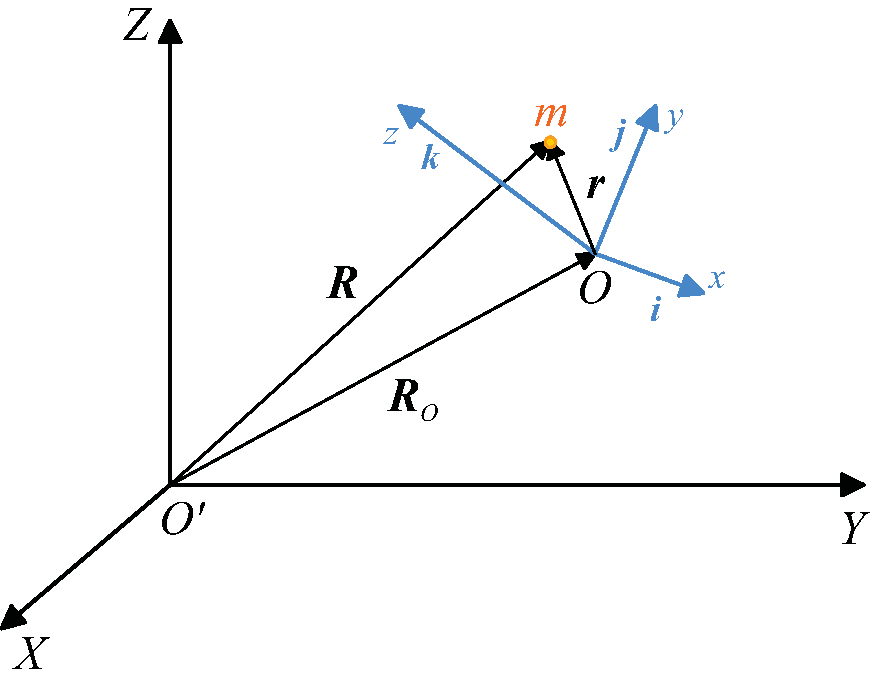
\includegraphics[width=0.4\linewidth]{pic/单质点角动量}
	\vspace*{-1em}
	\caption{质点$m$关于任意参考点$O$的角动量}
	\label{单质点角动量}
\end{figure}

在动坐标系中存在一个质量为$m$的质点,其\dy[线动量]{XDL}为
\begin{equation}
	\bm{p} = m \dot{\bm{R}}
	\nomenclature{$\bm{p}$}{质点的线动量 \nomrefpage}
\end{equation}
其中,$\bm{R}$为质点相对于惯性坐标系的位置向量(绝对位置向量)。

质点$m$的动量$\bm{p}$关于参考点$O$的\dy[角动量]{JDL}(或\dy[动量矩]{DLJ})定义为
\begin{equation}
	\bm{H}^O = \bm{r} \times m \dot{\bm{R}}
	\nomenclature{$\bm{H}^O$}{质点关于参考点$O$的角动量 \nomrefpage}
\end{equation}
其中,$\bm{r}$为质点$m$相对于参考点$O$的位置向量(相对位置向量)。由于$\bm{R} = \bm{R}_O + \bm{r}$,则有$\dot{\bm{R}} = \dot{\bm{R}}_O + \dot{r}$,那么
\begin{equation}
	\bm{H}^O = \bm{r} \times m \dot{\bm{r}} + \bm{r} \times m \dot{\bm{R}}_O
	\label{H1}
\end{equation}
其中,公式 \eqref{H1} 右侧第一项$\bm{r} \times m \dot{\bm{r}}$称为动坐标系$Oxyz$中的\dy[视角动量]{SJDL},用$\bm{H}^{\underline{O}}$表示;而另一项是因为点$O$运动引起的修正项。
\nomenclature{$\bm{H}^{\underline{O}}$}{质点的视角动量 \nomrefpage}

质点$P$关于参考点的角动量$\bm{H}^O$的时间导数(相对惯性系)为
\begin{align}
	\dot{\bm{H}}_O &= \dfrac{\d }{\d t} (\bm{r} \times m \dot{\bm{r}}) + m \dot{\bm{r}} \times \dot{\bm{R}}_O + m \bm{r} \times \ddot{\bm{R}}_O \notag \\[0.2em]
	&= \underbrace{\,\,\, \dfrac{\d }{\d t} (\bm{r} \times m \dot{\bm{r}}) \,\,\,}_{{\footnotesize \mbox{视角动量的变化率}}}  - \underbrace{ \,\,\, \ddot{\bm{R}}_O \times m \bm{r} \,\,\,}_{\footnotesize  \makecell[c]{\quad \\[-1.54em] \mbox{点}\, O \,\mbox{加速度的影响项}}} - \underbrace{\,\,\, \dot{\bm{R}}_O \times m \dot{\bm{r}} \,\,\,}_{\footnotesize  \makecell[c]{\quad \\[-1.54em] \mbox{点}\, O \,\mbox{速度的影响项}}}
\end{align}

\sssection[单质点的动量矩定理]

角动量$\bm{H}^O$的变化率可以与关于$O$点的外力矩联系起来。作用在$m$上的力关于点$O$的力矩定义为
\begin{equation}
	\bm{T}^O = \bm{r} \times \bm{F}
\end{equation}
\nomenclature{$\bm{T}^O$}{关于点$O$的力矩 \nomrefpage}
由牛顿第二定律,有
\begin{equation}
	\bm{F} = m \ddot{\bm{R}}
\end{equation}
所以
\begin{equation}
	\bm{T}^O = \bm{r} \times m \ddot{R} = \bm{r} \times m (\ddot{\bm{R}}_O + \ddot{\bm{r}})
\end{equation}
由于$\dot{\bm{r}} \times \dot{\bm{r}} = 0$,所以
\begin{equation}
	\bm{T}^O = \dfrac{\d }{\d t} (\bm{r} \times m \dot{\bm{r}}) - \ddot{\bm{R}}_O \times m \bm{r}
\end{equation}
而$\dot{\bm{H}}_O  =  \dfrac{\d }{\d t} (\bm{r} \times m \dot{\bm{r}} ) - \ddot{\bm{R}}_O \times m \bm{r} - \ddot{\bm{R}}_O \times m \bm{r}$,对比可得

\theorem[单质点的动量矩定理]{
	\index{DZDDDLJDL@单质点的动量矩定理}
	\index{DLJDL@动量矩定理}
	对于单质点$m$相对于任意参考点$O$的角动量$\bm{H}^O$与作用在$m$上的力关于点$O$的力矩$\bm{T}^O$的关系为
\begin{equation}
	\dot{\bm{H}}^O = \bm{T}^O - \dot{\bm{R}}_O \times m \dot{\bm{r}}
\end{equation}
特别地,如果参考点$O$是固定在惯性坐标系的一个点,那么$ \dot{\bm{R}}_O = 0$,即
\begin{equation}
	\dot{\bm{H}}^O = \bm{T}^O
\end{equation}
这就表明,如果外加力矩为0,那么$\bm{H}^O$就是常量,即在外力矩为0的条件下,质点的\dy[角动量守恒]{JDLSH}。
}

\clearpage

\subsection{多质点系统的动量矩定理}
如图 \ref{多质点角动量} 所示,假设坐标系$O'XYZ$是一个惯性坐标系,$O$是其中的一个动参考点,以$O$为原点建立一个动坐标系$Oxyz$。
\begin{figure}[!htb]
	\centering
	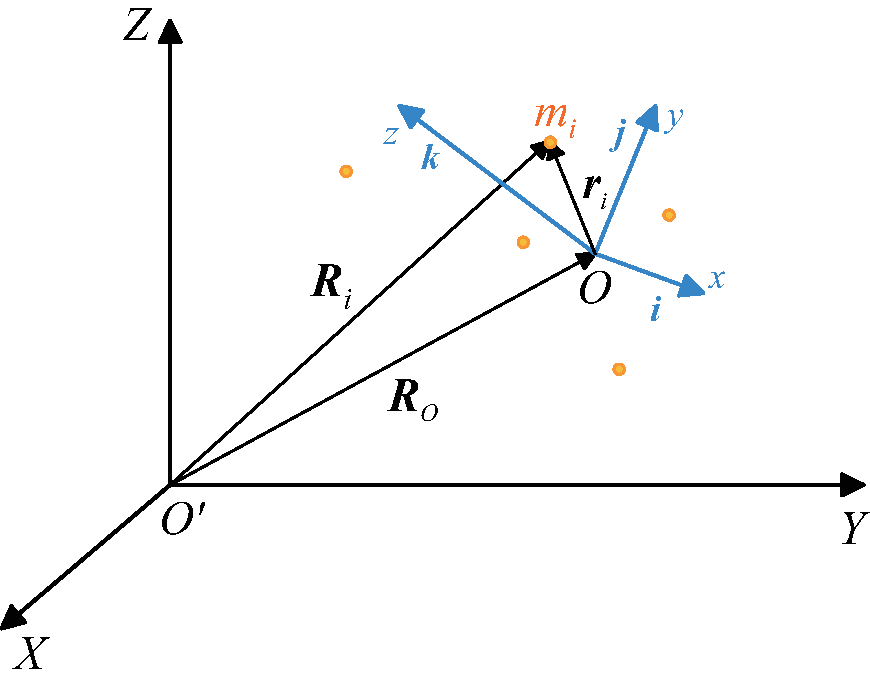
\includegraphics[width=0.4\linewidth]{pic/多质点角动量}
	\vspace*{-1em}
	\caption{某个质点$m_i$关于任意参考点$O$的角动量}
	\label{多质点角动量}
\end{figure}

在动坐标系中存在一个包含$N$个质点的多质点系统$A$,记第$i$个质点的质量为$m$,惯性系原点$O'$到这个质点的位置向量为$\bm{R}_i$,质点运动的绝对速度为$\bm{V}_i$。质点相对于动参考点的相对位置向量为$\bm{r}_i$,则有$\bm{R}_i = \bm{R}_O + \bm{r}_i$。

对于单个质点$m_i$其所受合外力为$\bm{F}_i$,那么其关于点$O$的力矩为$\bm{T}_i^O = \bm{r}_i \times \bm{F}_i$,那么整个质点系的外力关于$O$点的力矩为
\begin{equation}
	\bm{T}^O = \sum \bm{T}_i^O = \sum \bm{r}_i \times \bm{F}_i
\end{equation}

设多质点系统的总质量为$m = \displaystyle \sum m_i$,系统的总动量为$\bm{p} =  \displaystyle \sum m_i \bm{V}_i$,系统的质心为$C$,其绝对位置向量为$\bm{R}_C$,质心速度为$\bm{V}_C$,那么由单质点动量矩,单个质点$m_i$关于点$O$的动量矩为
\begin{equation*}
	\bm{H}_i^O = \bm{r}_i \times m_i \dot{r}_i - \bm{V}_O \times m_i \bm{r}_i
\end{equation*}
那么系统的动量矩为
\begin{equation}
	\bm{H}^O = \sum \bm{H}_i^O = \sum \bm{r}_i \times m_i \dot{\bm{r}}_i - \bm{V}_O \times \sum m_i \bm{r}_i
\end{equation}

\theorem[多质点系统的动量矩定理]
{
	与单质点关于动参考点的动量矩定理类似,多质点系统关于动参考点$O$的动量矩定理为
	\begin{align}
		\dot{\bm{H}}^O & = \sum \bm{T}_i^O - \bm{V}_O \times \sum m_i\dot{\bm{r}}_i \notag \\
		&= \bm{T}^O - \bm{V}_O \times \sum m_i (\bm{V}_O + \dot{\bm{r}}_i) \notag \\
		&= \bm{T}^O - \bm{V}_O \times \sum m_i \bm{V}_i \notag \\
		&= \bm{T}^O - \bm{V}^O \times \bm{p}
	\end{align}
可以看出,多质点系统关于动参考系的动量矩的时间导数不仅和外力矩有关,还与动参考点的平移运动以及系统的线动量有关,即{\color{dy} 多质点系统的姿态运动和平移运动耦合}。\\
\hspace*{2em} 特别地,当参考点$O$取质心$C$时,由牛顿第二定律及冲量定理,有\\[-1.7em]
\begin{equation}
	\dot{\bm{p}} = \sum \bm{F}_i  = m \dot{\bm{V}}_C
	\vspace*{-0.4em}
\end{equation}
积分后得系统动量的表达式:$\bm{p} = m \bm{V}_C$。而由于动参考点$O$取$C$,有$\bm{V}_O \times \bm{p} = \bm{V}_C \times \bm{p} = \bm{V}_C \times (m \bm{V}_C) = 0$,那么\\[-1.5em]
\begin{equation}
	\dot{\bm{H}}_C = \bm{T}^C
	\label{多质点动量矩}
\end{equation}
}
\clearpage
\vspace*{-2.5em}

\summarize
[
	\qquad 由多质点动量矩公式 \eqref{多质点动量矩} 可以看出,当系统质心$C$为参考点时,其动量矩定理具有和参考点取为固定点一样的简单形式,即{\color{dy}姿态运动和平移运动解耦}。这就是研究物体转动运动时常常取质心坐标系的原因。
]

























